\documentclass[tikz,border=8pt]{standalone}
\begin{document}
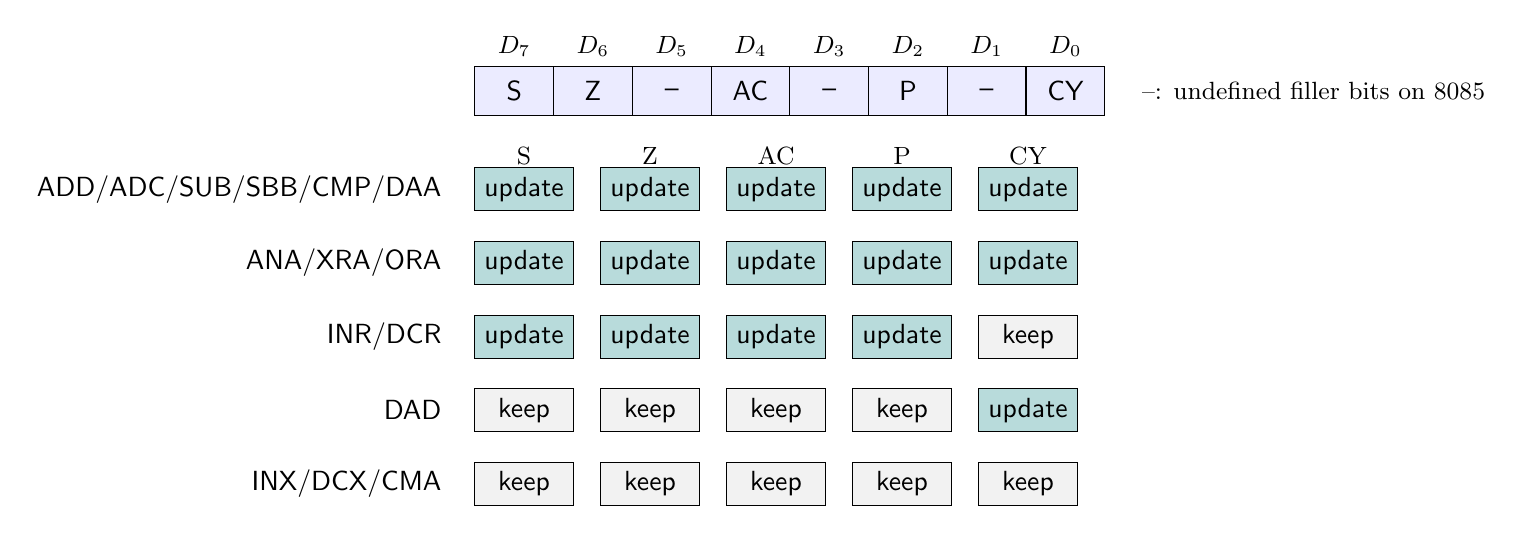
\begin{tikzpicture}[font=\sffamily,x=1cm,y=.78cm]
\foreach \x/\v in {0/S,1/Z,2/--,3/AC,4/--,5/P,6/--,7/CY}{\draw[fill=blue!8] (\x,6) rectangle ++(1,.8);\node at (\x+.5,6.4){\v};}
\foreach \x/\v in {0/$D_7$,1/$D_6$,2/$D_5$,3/$D_4$,4/$D_3$,5/$D_2$,6/$D_1$,7/$D_0$}{\node[font=\small] at (\x+.5,7.12){\v};}
\node[anchor=east] at (-.3,4.8){ADD/ADC/SUB/SBB/CMP/DAA};
\node[anchor=east] at (-.3,3.6){ANA/XRA/ORA};
\node[anchor=east] at (-.3,2.4){INR/DCR};
\node[anchor=east] at (-.3,1.2){DAD};
\node[anchor=east] at (-.3,0){INX/DCX/CMA};
\foreach \y in {4.8,3.6,2.4,1.2,0}{\foreach \x in {0,...,4}{\draw[fill=gray!10] (\x*1.6,\y-.35) rectangle ++(1.25,.7);\node at (\x*1.6+.625,\y){keep};}}
\foreach \y in {4.8,3.6}{\foreach \x in {0,...,4}{\draw[fill=teal!28] (\x*1.6,\y-.35) rectangle ++(1.25,.7);\node at (\x*1.6+.625,\y){update};}}
\foreach \x in {0,...,3}{\draw[fill=teal!28] (\x*1.6,2.4-.35) rectangle ++(1.25,.7);\node at (\x*1.6+.625,2.4){update};}
\draw[fill=teal!28] (4*1.6,1.2-.35) rectangle ++(1.25,.7);\node at (4*1.6+.625,1.2){update};
\foreach \x/\v in {0/S,1/Z,2/AC,3/P,4/CY}{\node[font=\small] at (\x*1.6+.625,5.35){\v};}
\node[font=\small,anchor=west] at (8.35,6.4){--: undefined filler bits on 8085};
\end{tikzpicture}
\end{document}
